\chapter{Magmatisme intrusif}
\label{chap1}
\minitoc

\section{Formation, transport et stockage des magmas}
\label{sec:magm-intr-un}

\subsection{Formation}
\label{sec:formation-1}

La majorité des magmas sont formées par fusion partielle des roches du
manteau  supérieurs.   Cependant,  dans  les  conditions  normales  de
pression,  la température  du manteau  supérieur n'est  pas suffisante
pour  provoquer la  fusion partielle  des roches  mantelliques (Figure
\ref{Geoterme}) et  d'autres mécanismes  sont nécessaires  pour amener
les roches  du manteau à croiser  leur liquidus.  Au niveau  des zones
d'extension, i.e. au niveau des  dorsales océaniques par exemple ou au
sein des  panaches mantelliques, la  fusion partielle est  ainsi causé
par décompression  des roches  mantelliques.  Au  niveau des  zones de
subduction, les mécanismes  mises en jeux sont plus  complexes et font
intervenir la  déshydratation par  chauffage des roches,  la migration
des fluides provoquant la fusion des roches alentours.

\begin{figure}[h!]
  \begin{center}
    \graphicspath{ {/Users/thorey/Documents/These/Manuscript/Figure/Chapter1/} }
    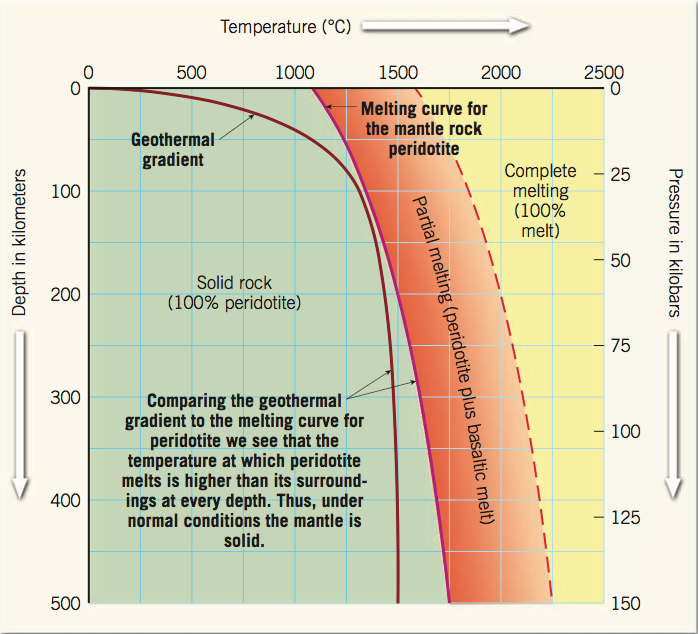
\includegraphics[scale=0.4]{geoterme.png}
    \caption{Temperature ($\°C$)  versus depth (km).   Reproduced from
      \citet{Tarbuck:1998ud}.}
    \label{Geoterme}
  \end{center}
\end{figure}

\subsection{Transport}
\label{sec:transport}

Les liquides de  fusions ainsi formés sont moins dense  que les roches
solides alentours et s'élèvent donc,  par compaction et percolation au
travers          de           la          matrice          mantellique
\citep{McKenzy:1984bo,McKenzie:1985jq}. Le magma,  liquide de fusion +
cristaux, s'accumule ensuite au sein de  chenaux, i.e.  de dykes ou le
long  de  faille  pré-existantes  pour remonter  rapidement  vers  les
couches          superficielles          de         la          croûte
\citep{Lister:1991ut,Clemens:1992kr,Petford:1993bk,Rubin:1995upa}.  En
effet, bien  que l'idée du magma  remontant lentement au sein  de gros
volume  diapirique est  encore  parfois  invoqué au  sein  de la  base
ductile  de  la   croûte  \citep{Weinberg:1994jg,Weinberg:1996vb},  le
transport rapide  du magma  au sein  des dykes  permet de  résoudre de
nombreux problèmes,  thermiques et  mécaniques, associés à  la remonté
diapirique  de gros  volume de  magma au  sein des  parties supérieurs
fragiles de la croûte invoquée historiquement \citep{Miller:1999km}.

\subsection{Stockage}
\label{sec:stockage}

Historiquement, les  travaux de  \citet{Walker:1989jq} ont  montré que
les  magmas  remontent jusqu'à  rencontrer  leur  zone de  flotabilité
neutre, une région ou la densité de la roche encaissante est proche de
celle du magma lui même. En effet, au dessus de cette couche, le magma
est plus dense  que la roche encaissante et  sa flotabilité l'entraîne
vers    le    bas.     De   nombreux    travaux,    tant    théoriques
\citep{Lister:1991ut,Petford:1993bk,Rubin:1995upa}  que  expérimentaux
\citep{Taisne:2009kj,Taisne:2011do}  ont en  effet  depuis montré  que
l'ascension  d'un dyke  était contrôlé  par la  différence de  densité
entre la  tête de celui  ci et la  roche encaissante. Lorsque  le dyke
entre dans  une région de  densité inférieure, la  surpression induite
peut, sous  certaines conditions, conduire  à l'étalement du  magma au
niveau   de   la  base   de   la   région   de  plus   forte   densité
\citep{Taisne:2011do}. Le magma s'étale donc  par gravité à la base de
cette  couche permettant  ainsi la  formation de  réservoir magmatique
sous forme d'intrusion magmatique au sein de la croûte. L’existence et
la  localisation de  cette zone  de  flottabilité neutre,  et donc  la
question de l'éruptabilité  d'un magma, dépend de  la densité relative
entre la  croûte et le  magma.  Elle dépend  donc non seulement  de la
nature  de la  croûte,  i.e.   de sa  composition,  mais  aussi de  sa
porosité,  de la  composition du  magma, de  sa température  et de  sa
teneur en volatils, qui varie, elle,  largement avec la pression et la
profondeur.

Plus  récemment, d'autres  études  ont montré  que  les contrastes  de
rigidité  entre les  différentes  couches  crustales pourraient  aussi
jouer un  rôle non  négligeable sur l'arrêt  de l'ascension  des dykes
\citep{Menand:2011ki}.   En  effet,   des  expériences  réalisées  par
\citet{Kavanagh:2006ig} ont  montré que la propagation  d'un dyke peut
être  arrêté quand  celui ci  rencontre  une interface  qui sépare  un
milieu  plus  rigide  surplombant   un  milieu  moins  rigide  (Figure
\ref{Neutral_Zone}). Le  dyke arrête ainsi son  ascension verticale et
s'étale horizontalement juste en dessous de la couche de rigidité plus
élevée. Ce  mécanisme est d'autant  plus efficace que le  contraste de
rigidité est important \citep{Kavanagh:2006ig}.

\begin{figure}[h!]
  \begin{center}
    \graphicspath{ {/Users/thorey/Documents/These/Manuscript/Figure/Chapter1/} }
    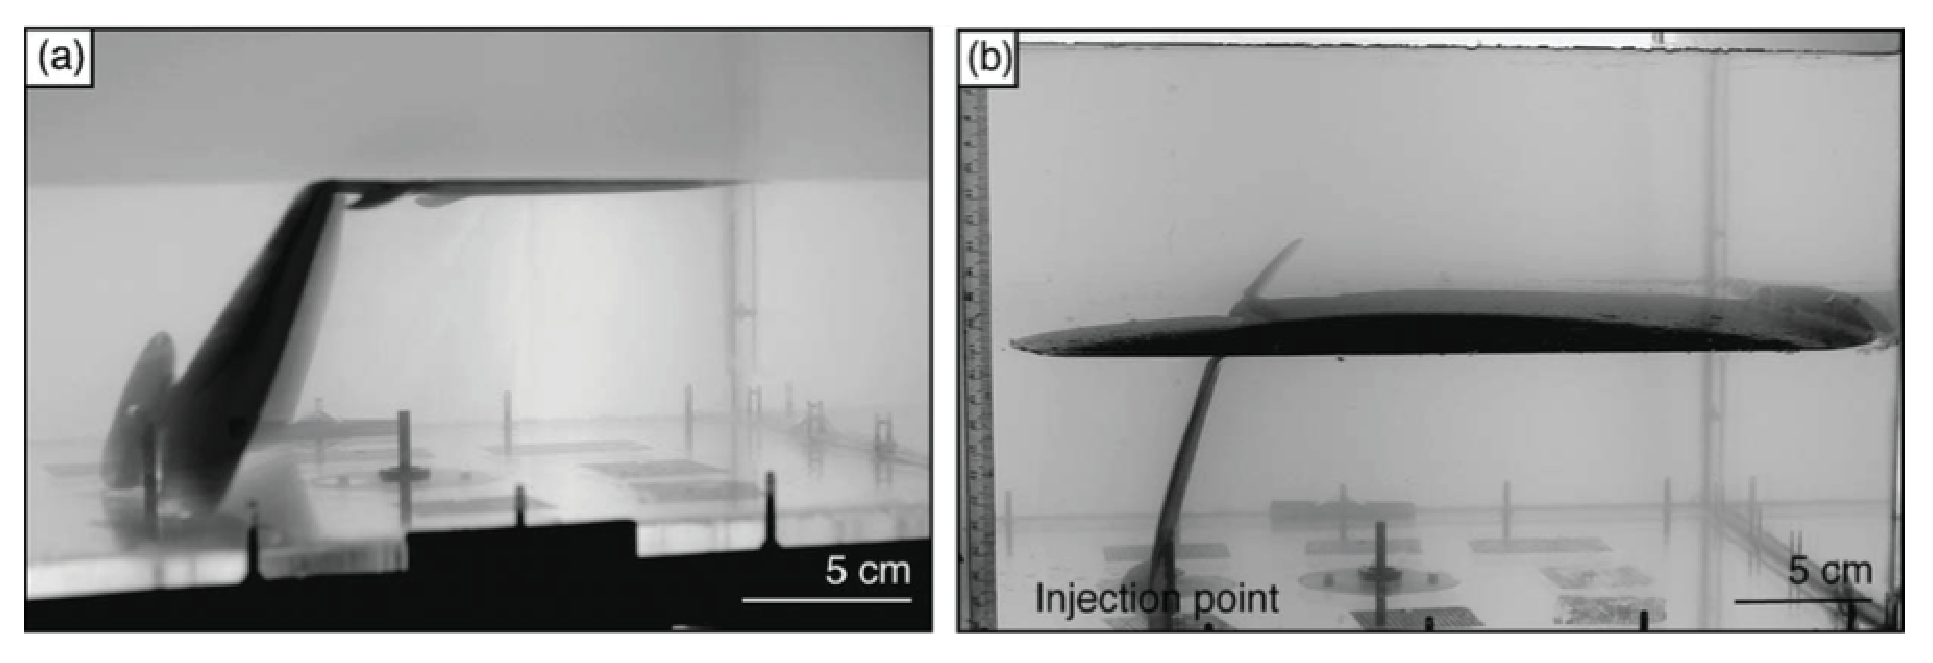
\includegraphics[scale=0.4]{Neutral_Zone.eps}
    \caption{a)  Photographie de  deux des  expériences réalisées  par
      \citet{Kavanagh:2006ig}   sur  le   comportement  d'un   dyke  à
      l'interface entre  deux milieux de rigidités  différentes. a) Le
      contraste de rigidité est très important et le dyke s'étale sous
      la couche de  rigidité importante.  b) Le  contraste de rigidité
      est plus faible et, tout en s'étalant en dessous de la couche de
      rigidité  supérieur, le  dyke  continue sa  progression dans  le
      milieu plus rigide.}
    \label{Neutral_Zone}
  \end{center}
\end{figure}


Finalement, les contraintes, locales ou globales, peuvent aussi dévier
la trajectoire d'un dyke et influencer  les trajets des magmas au sein
de la  croûte.  En  effet, des  études ont  montré que  les intrusions
magmatiques tendent  à se propager perpendiculairement  à la direction
des contraintes de  compressions \citep{Anderson:L5JA3dNN}.  Les dykes
ont donc tendance à exister dans  des situations ou les contraintes de
compressions sont horizontales  et donc à s'arrêter quand  le champ de
contrainte  évolue,  d'une  contrainte  de  compression  horizontal  à
vertical  comme  c'est le  cas  par  exemple  au niveau  des  édifices
volcaniques \citep{Pinel:2000wa,Pinel:2004ji,Roman:2014hw}.

Cependant, si  ces différents  facteurs jouent  sûrement tous  un rôle
dans  le transport  et le  stockage des  magmas au  sein de  la croûte
terrestre, la densité relative du magma et de la roche encaissante est
certainement le facteur déterminant dans  la mise en place d'intrusion
magmatiques et  la structure en  densité d'une croûte  planétaire joue
donc un rôle essentielle dans le stockage des magmas.

\section{Caractérisation du  magmatisme intrusif à  faible profondeur:
  apport des observations}
\label{sec:zool-des-intr}

\subsection{Intrusion magmatique sur Terre}
\label{sec:definition}

La croûte terrestre continentale, épaisse en moyenne de $35$ km, a une
densité  moyenne proche  de $2900$  kg m$^{-3}$.   De part  sa densité
relativement basse, elle constitue un filtre efficace à la remonté des
magmas en surface qui  sont par conséquence préférentiellement stockés
en profondeur.  \citet{Crisp:1984dm}  et \citet{White:2006gr} estiment
en effet à  $10$ fois supérieur au volume de  lave extrudé les volumes
de magma intrudés  au sein de la croûte  continentale.  Les mouvements
tectoniques  au sein  de  la  croûte ainsi  que  l’érosion ont  exposé
nombreuses  de ces  intrusions magmatiques  à la  surface. La  mise en
place  ces  magmas  en  profondeurs et  leur  solidification  semblent
résulter en une grande variété  de morphologie et de type d'intrusions
différentes dépendante des conditions, profondeurs et caractéristiques
mécaniques du milieu encaissant au moment de la formation.

Les batholiths  sont de  loin les plus  imposants représentant  de ces
familles  d'intrusions  magmatiques.   Ils peuvent  atteindre  jusqu'à
quelques  kilomètres d'épaisseur  et  s'étendre sur  des centaines  de
kilomètres.   Par  exemple, le  batholith  de  Sierra Nevada  est  une
intrusion granitique qui s'étend sur  presque la totalité de la Sierra
Nevada en Californie.  Il est maintenant clair que la mise en place de
ces gigantesques volumes de magmas  se forme par incréments successifs
de petits  volume de magma se  solidifiant lors de leur  mise en place
sur   de  longues   échelle   de  temps   $10^5$   to  $10^6$   années
\citep{Petford:2000cc,Glazner:2004gv}. Dans cette thèse, on va donc se
focaliser sur  les mécanismes de  formations et  de mise en  places de
plus  petit volume  de  magma  dans la  partie  fragile  de la  croûte
continental, des profondeurs inférieurs à $10$ km. The intrusive suites of the Tuolumne and Mt. Stuart Batholiths have ages that span between ten and five million years (Coleman et al., 2004; Matzel et al., 2006), which is longer than cooling models allow for a large single magma chamber to exist in

492 S. Morgan et al. / Journal of Structural Geology 30 (2008) 491e512
the middle  to upper crust (Glazner  et al., 2004). The  incremen- tal
assembly  model of  pluton emplacement  is also  consistent with  dike
transport  of magma,  which is  now commonly  invoked as  the dominant
mechanism of magma ascent through  the middle and upper crust (Clemens
and Mawer, 1992; Petford, 1996).

Rajotuer ca

On  distingue généralement  deux types  d'intrusions magmatiques:  les
intrusions discordantes, qui se mettent en place perpendiculairement à
la   stratification  naturelle   de  la   croûte  et   les  intrusions
concordantes,  qui  se  mettent  en  place  parallèlement  aux  couche
géologiques. Des études géologiques de  terrain ont montré la présence
de   quatre  grandes   familles  d'intrusions   magmatique  à   faible
profondeur.

\begin{figure}[h!]
  \begin{center}
    \graphicspath{ {/Users/thorey/Documents/These/Manuscript/Figure/Chapter1/} }
    \includegraphics[scale=0.5]{Intrusive_Activity.eps}
    \caption{a) Différentes formes  du magmatisme intrusif: batholith,
      dyke,  sill   et  laccolith.    Dimensions  typiques   pour  des
      laccoliths,   dyke  et   sill  de   composition  et   d'origines
      différentes repris de \citet{Cruden:tg}. }
    \label{Dimension}
  \end{center}
\end{figure}

\begin{itemize}
\item  Les  dykes,  par  lesquels  remontent le  magma  à  travers  la
  lithosphère sont discordants et  caractérisé par de faibles rapports
  d'aspects (Figure \ref{Dimension}, \ref{picture} a).  Leur épaisseur
  peut  varier  de quelques  mètres  à  quelques centaines  de  mètres
  d'épaisseur      \citep{Walker:1989jq,Rubin:1995upa},     cependant,
  l'épaisseur moyenne est de quelques  dizaines de mètre. Les dykes de
  compositions felsiques  sont généralement  plus épais et  moins long
  que leurs équivalents mafiques \citep{Rubin:1995upa}.

\item Les sills,  à la différence des dykes,  sont concordants (Figure
  \ref{Dimension},  \ref{picture} b,f).   Ils se  mettent en  place le
  long de discontinuités  ou de failles pré-existantes,  à la jonction
  entre  deux  couches  sédimentaires  par  exemple.   Les  sills  aux
  dimensions les plus importantes répertoriés sont mafiques et peuvent
  attendre  jusqu'à $100$  km sur  des  épaisseurs de  presque $1$  km
  \citep{Cruden:tg}.   Leurs homologues  felsiques,  plus rares,  sont
  souvent de dimension plus raisonnable.

  \begin{figure}[h!]
    \begin{center}
      \graphicspath{ {/Users/thorey/Documents/These/Manuscript/Figure/Chapter1/} }
      \includegraphics[scale=0.95]{photo.eps}
      \caption{a) Dyke  traversant des  couches sédimentaires  dans le
        Makhtesh  Ramon,  Israel;  b)   Sill  basaltique  au  sein  de
        sédiments, vallée  de la  Yellowstone River, Parc  National du
        Yollowstone  (USA).   Photographie  de  Fabrice  Pinchon.   c)
        Laccolith   à  l'érosion   dans  le   Montana  d)   Schéma  de
        l'emplacement       d'un      laccolith       réalisé      par
        \citet{Gilbert:1877uk}. e) Schéma simplifié de la structure en
        arbre de noel d'un complexe  de laccolith sur l'île d'elbe, en
        Italie,  étudié par  \citet{Rocchi:2010dn}.   f) Intrusions  à
        l'érosion au alentour  de la montagne Hillers,  dans les Henry
        Mountains.   On peut  distinguer  le black  Mesa bysmalith  au
        centre et  le Maiden Creek  sill en dessous.   Photographie de
        Jack Share}
      \label{picture}
    \end{center}
  \end{figure}

\item    Les   laccoliths    ont   été    décrit   premièrement    par
  \citet{Gilbert:1877uk}  suite  à  son  étude  géologique  des  Henry
  Mountains, dans  l'Utah aux  Etats-Unis (Figure \ref{picture}  c, d,
  e).  Ils se mettent en  place principalement par flexion des couches
  sédimentaires sus-jascentes, ce  qui leur donnent une  forme plus ou
  moins en  cloche.  \citet{E:2015tl}  a répertorié  à peu  près $900$
  laccoliths,  principalement  dans  le nord  des  Etats-Unis.   Leurs
  épaisseurs  varient de  quelques  dizaines à  quelques centaines  de
  mètres et leurs  rayons peut atteindre quelques  kilomètres pour les
  plus  gros  (Figure  \ref{Dimension}  b).  Ces  laccoliths  se  sont
  parfois mis en place les uns sur les autres formant une structure en
  forme d'arbre  de noël \citep{E:2015tl}.  Cette  géométrie est aussi
  observé  sur  l'île  d'Elbe,  en  Italie, ou  un  complexe  de  neuf
  laccoliths, exceptionnellement bien conservé, a été étudié en détail
  par \citet{Rocchi:2002jy}. De nombreux  laccoliths sont aussi marqué
  par un toit  plat, la flexure de l'encaissant ne  concernant que les
  flans du laccolith \citep{Koch:1981if}.

\item   Les   bysmaliths   sont  d'imposants   volumes   cylindriques,
  préférentiellement composé  de roche granitique,  discordant (Figure
  \ref{picture}  f).   Ils  sont notamment  bordés  par  d'importantes
  failles quasiment verticales et peuvent atteindre quelques centaines
  de mètre  d'épaisseur \citep{Johnson:1973ho}. Un exemple  typique de
  ce  type d'intrusion  est le  Black  Mesa Bysmalith  dans les  henry
  mountain, $200$ m d'épassieur et $1$ km de large \citep{Morgan:2008hj}.
\end{itemize}

A  l'instar des  batholiths,  de nombreuses  observations de  terrains
proposent que  les intrusions de  taille moyenne se forment  aussi par
incrément     successif     de      petit     volume     de     magmas
\citep{Habert:2004wg,Horsman:2005ct}      (Figure     \ref{Horsmann}).
Cependant,  les  même études  montrent  aussi  que ces  intrusions  se
forment sur de petite échelle de  temps, une échelle assez petite pour
pouvoir  garder  un corps  chaud  et  liquide  des première  étape  du
processus d'intrusion à  sa solidification. Au niveau  du bysmalith de
Black Mesa par exemple (Figure \ref{picture} f), \citet{Habert:2004wg}
ont montré l'absence de structures entre les différentes couches ainsi
que l'absence  de métamorphisme important dans  l'encaissant supposant
un temps de mise en place de moins de $100$ ans.

\begin{figure}[h!]
  \begin{center}
    \graphicspath{ {/Users/thorey/Documents/These/Manuscript/Figure/Chapter1/} }
    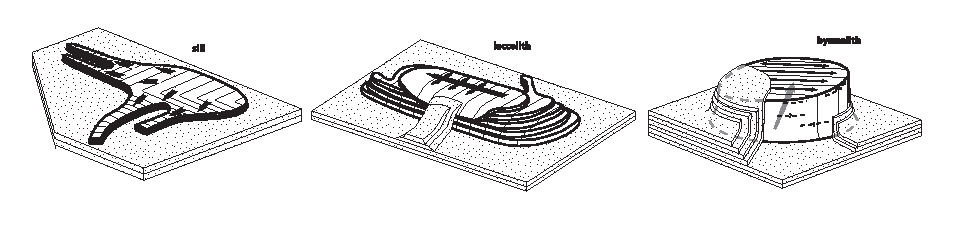
\includegraphics[scale=0.8]{Horsmann.eps}
    \caption{Ces  diagrammes,  réalisés  par  \citet{Horsman:2009gea},
      montrent la structure verticale en  couche de trois intrusions à
      l'érosion  dans les  Henry  mountains. De  gauche  a droite:  le
      Maiden  Creek sill  (Figure \ref{picture}  f), le  Trachyte Mesa
      laccolith et le black mesa bysmalith (Figure \ref{picture} f).}
    \label{Horsmann}
  \end{center}
\end{figure}

Parler aussi du papier de \citep{Roni:2014gt}. The lack of internal discontinuities indicates that the magma was injected as a single pulse or a series of quickly coalescing pulses.
\subsection{Intrusion magmatique sur la Lune}
\label{sec:moon}

La densité de la croûte lunaire est particulièrement faible, $2550$ kg
m$^{-3}$ selon  les dernières  estimations faite  à l'aide  des donnés
gravitaires de  la mission GRAIL de  la NASA\citep{Wieczorek:2013ipa}.
La  porosité   résultante  de  4  milliard   d'année  de  bombardement
météoritique, qui  pourrait être  de l'ordre de  $12\%$, ainsi  que la
faible  densité   des  minéraux   la  composant,   principalement  des
plagioclases, tous les  deux contribuent à sa  faible densité. D'autre
part, l'épaisseur  de la croûte  n'est pas négligeable, entre  $34$ et
$43$ km en moyenne  avec une tendance à être plus  épaisse sur la face
cachée que sur la face visible.

La faible  densité de sa crôute  et son épaisseur non  négligeable ont
certainement joué  un rôle  important sur  le volcanisme  lunaire.  En
effet, les  laves extrudés au  sein des  mers lunaires sont  riches en
éléments lourd,  fer principalement  $FeO$ et  titan $TiO_2$,  et sont
caractérisés par  des densités  de l'ordre de  $3000$ kg  m$^{-3}$. La
faible densité de la croûte a donc sans doute jouait aussi sur le Lune
le  rôle d'un  filtre efficace  à l'extrusion  des magmas,  formés par
fusion partielle de son manteau,  en surface, leur flotabilité ne leur
permettant        pas        généralement        d'atteindre        la
surface. \citet{Head:1992bk} ont estimé ainsi à 50 fois plus important
aux volumes  extrudé en surface le  volume des magmas intrusif  sur la
lune.   Cependant, bien  que ce  rapport puisse  donner de  précieuses
indications sur l'évolution thermique de la  lune elle même, il est de
fait très  peu contraints.  La  détection des déformations  de surface
induites par  la mise en  place d'intrusion  magmatique au sein  de la
croûte  permet une  meilleur  caractérisation  du magmatisme  intrusif
lunaire.

Deux  manifestations principales  à  la  surface de  la  lune ont  été
proposé  comme   potentiellement  résultant   de  la  mise   en  place
d'intrusions magmatiques  au sein  de la croûte  lunaire: les  domes à
faible pente et les cratères au sol fracturé.

\begin{itemize}
\item Les  domes à faible pente  sont localisé en bordure  ou dans les
  mers   lunaires,  principalement   sur  la   face  visible   (Figure
  \ref{Moon-magma} a, b).  $13$ de  ces domes ont été recemment décrit
  par \citet{Wohler:2007it}.  Bien que  leur morphologie s'apparente à
  des laccoliths terrestres, ils sont de manière général beaucoup plus
  étalés que  ceux sur  Terre; pour  une même  épaisseur, l'équivalent
  lunaire  peut ainsi  être deux  fois plus  larges que  son homologue
  Terrestre.

  \begin{figure}[h!]
    \begin{center}
      \graphicspath{ {/Users/thorey/Documents/These/Manuscript/Figure/Chapter1/} }
      \includegraphics[scale=0.95]{Moon_Lacc.eps}
      \caption{a)  Dome lunaire,  photo  par Appolo  17  b) Apollo  15
        orbital image  AS15-91-12372, vue  oblique du  dôme Valentine.
        c) Cratère au sol fracture Atlas (Classe 1). d) Cratère au sol
        fracturé  Lavoisier (Classe  5).  e)  Cratère au  sol fracturé
        Gassendi  (Classe  3).  f)  Cratère  au  sol fracturé  Komarov
        (Classe   5).   Photo   extraite   de  \textit{Lunar   Orbiter
          Photographic Atlas of the Moon, NASA}}
      \label{Moon-magma}
    \end{center}
  \end{figure}

\item Les  cratères à sol  fracturé sont des cratères  d'impacts ayant
  subis des déformations suite à leur formation.  A peu près $ 200$ de
  ces   cratères  ont   été  répertorié   par  \citet{Schultz:1976kt},
  principalement autour des mers  lunaires (Figure \ref{Moon-magma} c,
  d, e,  f).  La principale  caractéristique de ces cratères  est leur
  faible profondeur  par rapport à  celles des cratères  non déformés.
  En effet, certain  cratère au sol fracturé peuvent  être jusqu'à $2$
  km moins profond que leurs homologues non déformées.  Leur sol, soit
  en  forme de  dôme, soit  plat séparé  des mures  du cratère  par un
  imposant  fossé  circulaire,  est systématiquement  caractérisé  par
  d'important réseaux  de fractures radiales, concentriques  ou encore
  pentagonales (Figure  \ref{Moon-magma} c, d,  e, f).  Basé  sur leur
  profondeur,     topographie     et    niveau     de     déformation,
  \citet{Schultz:1976kt} a postuler l'existence  de six grandes classe
  de  déformation.   La  proximité  des ces  cratères  avec  les  mers
  lunaire, ainsi  que la présence  de produits volcaniques au  sein de
  certain cratère, suggèrent qu'ils ont été déformé suite à la mise en
  place de magma en profondeur sous leur sol.
\end{itemize}

\subsection{Intrusions   magmatiques    sur   les    autres   planètes
  telluriques}
\label{}


\section{Caractérisation du  magmatisme intrusif à  faible profondeur:
  apport de la modélisation}
\label{sec:orign-theor-fram}

\subsection{Model statique de déformation d'une couche élastique}
\label{sec:model-statique-de}

Bien que la  tailles, la morphologie et les volumes  de magmas mise en
jeux peuvent  être récupérés,  à partir  d'observations directs  ou de
méthodes de prospection géophysique sur Terre, ou via les déformations
induites  à  la surface  des  autres  corps  du système  solaire,  ces
informations seuls ne donnent que  peu d'indication sur les mécanismes
de  mise  en  place  de  ces intrusion  magmatiques.   En  effet,  ces
observations  doivent  être interprété  sous  le  regards des  modèles
d'intrusion magmatiques pour pouvoir  extraire des informations sur le
processus d'intrusion lui même, i.e.   sur les paramètres physiques du
magma, les taux d'injection ou encore la profondeur de mise en place.

La propagation  d'un dyke dans un  milieu élastique a été  décrite par
\citep{Lister:1991ut,Rubin:1995upa}.           En         particulier,
\citet{Lister:1990hz} ont montré que, à  l'exeption de la tête du dyke
où  les contraintes  élastiques induites  par les  roches encaissantes
jouent un  rôle important, la dynamique  du magma au sein  du dyke est
contrôlée  par  un  équilibre  entre  la  flotabilité  et  les  pertes
associées à la viscosité du magma lui même. On a vu qu'un dyke peut se
transformer  en sill  si celui  ci  rencontre sa  zone de  flotabilité
neutre. La  dynamique des dykes  et des  sills est comparable  à forte
profondeur   \citep{Lister:1991ut,Cruden:tg},   cependant,  à   faible
profondeur,  la  forme  des  laccoliths supposent  que  les  intrusion
magmatiques se mettent en place principalement par flexion des couches
sédimentaires  sus-jacentes \citep{Johnson:1973ho}.   Les plupart  des
travaux  modélisant  ces  intrusions  magmatiques  utilisent  donc  la
théorie linéaire  de l'élasticité qui  prédit la flexure  d'une plaque
élastique en fonction de la  contrainte appliqué (le taux d'injection)
et     des     caractéristiques     mécaniques     de     l'encaissant
\citep{Pollard:1973ho,Koch:1981if}. Ces travaux  ont par exemple était
appliqué à certain laccolith dans  les Henry Mountains et pour déduire
les  profondeur  d'intrusion et  les  taux  d'injection nécessaire  au
niveau des dômes lunaires \citep{Wohler:2007it} et des cratères au sol
fracturés \citep{Jozwiak:2012dq}.

\subsection{Emplacement dynamics des sills  et laccoliths: que peut on
  apprendre de leur géométrie ?}
\label{sec:empl-dynam-des}

Ces  modèles  statiques  ne  fournissent  aucune  information  sur  la
dynamique du processus d'intrusion et sont donc incapables d'expliquer
la diversité des formes observées. De plus, ils négligent la viscosité
des  magmas ainsi  que  le  propre poids  de  l'intrusion qui  doivent
nécessairement jouer un rôle sur la  mise en place de l'intrusion.  En
l'absence  d'un   modèle  dynamique  d'intrusion,  la   géométrie  des
intrusions répertoriées a été utilisé  pour en déduire des indications
sur les processus de mise en place et de croissance de ces intrusions.
Ainsi,  en utilisant  les donnés  répertoriés sur  les laccoliths  par
\citet{E:2015tl},   \citet{McCaffrey:1997ea}   propose  une   loi   de
puissance empirique pour l'épaisseur  des intrusions $h_0$ en fonction
de leur longueur $R$, $h_0 = bR^a$  ou $a$ est l'exposant de la loi de
puissance et  $b$ une  constante. Ainsi, un  exposant supérieur  à $1$
indique que l'intrusion croit  préférentiellement en s'épaississant et
un  exposant  inférieur  à  $1$   indique  qu'elle  croit  plutôt  par
étalement.

\begin{figure}[h!]
  \begin{center}
    \graphicspath{ {/Users/thorey/Documents/These/Manuscript/Figure/Chapter1/} }
    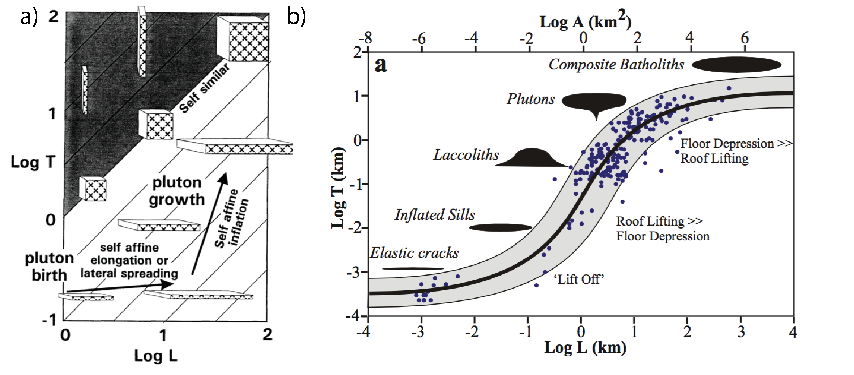
\includegraphics[scale=0.95]{Model.pdf}
    \caption{a)  Schéma de  la formation  des laccoliths  suivant deux
      étapes   par   \citet{McCaffrey:1997ea}.    Nouvelles   données:
      épaisseurs  en  fonction de  leur  longueur  de différent  types
      d'intrusions  magmatiques   à  différentes   locations.   Figure
      extraite de \citet{Cruden:tg}.}
    \label{Model}
  \end{center}
\end{figure}

Les laccoliths  répertoriés par \citep{E:2015tl} montrent  un exposant
$a<1$  ($0.88  \pm 0.1$)  interprété  comme  reflétant l'étalement  de
l'intrusion sur une  certaine distance sous forme d'un  sill avant son
épaississement (Figure  \ref{Model}).  Ce modèle est  cohérent avec le
modèle couramment accepté pour la mise  en place des laccolith en deux
étapes   \citep{Johnson:1973ho,McCaffrey:1997ea}.   Premièrement,   le
magma s'étale latéralement au niveau  de sa zone de flotabilité neutre
$a<1$  jusqu'à ce  qu'un  sill  soit formé  caractérisé  par un  large
rapport  d'aspect.   Ensuite,  lors  de la  deuxième  étape,  le  sill
s'épaissit  par  flexion  des  couches sus-jascentes  pour  former  un
laccolith  caractérisé  par $a>1$  \citep{Johnson:1973ho,Koch:1981if}.
Si la roche sus-jacente est soumise à des contraintes trop importante,
des  failles se  forment au  niveaux  des bords  du sill  et celui  ci
s'épaissit  uniformément sur  toute  sa surface  formant un  bysmalith
\citep{E:2015tl}.   L'étude détaillée  du complexe  intrusif de  l'île
d'Elbe en  Italie (Figure  \ref{Rocchie_Schema}) montre  des exposants
supérieur  à $1$,  jusqu'à $1.5$  interprété comme  étant le  résultat
d'une croissance dominé par l'épaississement de l'intrusion.

Des modèles plus récent conçoivent  plutôt la formation des laccoliths
par empilement successif de sill  de grand rapport d'aspect plutôt que
par  injection   d'un  volume   de  magma  fini   à  un   temps  donné
\citep{Menand:2011ki}.   En effet,  ces  modèles sont  en accord  avec
expérience de \citep{Kavanagh:2006ig}  (Section \ref{sec:stockage}) où
les  sills  se mettent  en  place  à  l'interface entre  deux  couches
rigidité différentes, la rigidité de la couche sus-jascente étant plus
importante que celle de la couche sous-jascente.  En effet, la mise en
place d'un sill en refroidissant  procure un environnement favorable à
la mise en place d'un nouveaux sill,  soit au dessus si la rigidité du
sill solidifié  est inférieur à celle  de la roche sus-jascente  ou en
dessous. Ce modèle  de croissance est supporté par  de récentes études
structurales et  stratigraphiques, notamment au niveau  des intrusions
de     taille    intermédiaires     dans    les     Henry    Mountains
\citep{Horsman:2005ct,Morgan:2008hj,Horsman:2009gea,Menand:2011ki}. Ce
modèle permet aussi de rendre compte de la structure plate du toit des
laccoliths.   Cependant, ce  mécanisme  de croissance  ne devrait  pas
impliquer  un   exposant  caractéristique  de  la   géométrie  de  ces
laccoliths.

\citet{Nachwuchskoechin:2002tv}  ont réunit  des donnés  sur une  plus
grande plage  de longueurs,  des petits  cracks élastique  de quelques
dizaines de mètres aux battholith  de quelques centaines de kilomètres
(Figure  \ref{Model}).  \citep{Nachwuchskoechin:2002tv}  proposent que
l'épaisseur en fonction de la longeur des intrusions magmatiques forme
une   distribution  en   forme  de   sigmoide  (   dans  une   échelle
logarithmique) avec  une pente  maximum de $1.5$  caractéristiques des
laccoliths.   Cependant, aucune  théorie sous-jascente  soutient cette
observation. De plus, les données  de \citep{Cruden:tg} sur les larges
sills   mafiques   contredise   cette  vision   des   choses   (Figure
\ref{Dimension}).

\section{Discussion}
\label{sec:discussion}

En conclusion, aucun des modèles  présentés plus haut n'est cohérent à
la  fois avec  la morphologie  des sills  et des  laccoliths et  leurs
rapport  d'aspect.  Dans  le  but  de comprendre  plus  en détails  la
dynamique de l'intrusion, \citet{Michaut:2011kg} a développé un modèle
théorique d'étalement  d'un magma  visqueux sous une  couche élastique
d'épaisseur contant continuellement nourrit par un conduit vertical en
son centre. Ce  modèle diffère de ces prédecesseurs par  sa capacité a
traité la  dynamique même de l'intrusion  ainsi que le poids  du magma
comme un moteur  de l'écoulement. Ce modèle a été  développé en 2D par
\citep{Thorey:2014cv}. Dans  la suite,  je présente  le modèle  et les
résultats que nous avons obtenus dans une géométrie axisymmétrique.


\bibliographystyle{agufull08}
\bibliography{/Users/thorey/Dropbox/Library}

%%% Local Variables:
%%% mode: latex
%%% TeX-master: "../main"
%%% End:
